%\documentclass[aps,twocolumn,floatfix,prl]{revtex4-1}
%\documentclass[letterpaper,10pt,prl,twocolumn,aps]{revtex4-1}
\documentclass[aps,preprint,floatfix,prl]{revtex4-1}
\usepackage{fullpage}
\usepackage{amsmath}
\usepackage{amsfonts}
\usepackage{amssymb}
\usepackage{graphicx}
\usepackage{slashbox}
\usepackage{color}
\usepackage{longtable}
\usepackage{array}
\usepackage{dashrule}

\usepackage{amsmath}

\usepackage{dcolumn}% Align table columns on decimal point

\usepackage{graphicx}% Include figure files
\usepackage{dcolumn}% Align table columns on decimal point
\usepackage{bm}% bold math
\usepackage{ifthen}
\usepackage{amsthm} % Theorem Formatting
\usepackage{amssymb}	% Math symbols such as \mathbb
\usepackage{calrsfs}
\graphicspath{ {images/} }

\newcommand{\ellcap}{{\ell_\text{c}}}
\newcommand{\Fh}{{\boldsymbol{F}_h}}
\newcommand{\Fv}{{\boldsymbol{F}_v}}
\newcommand{\Tv}{{\boldsymbol{T}}}
\newcommand{\bn}{{\boldsymbol{n}}}
\newcommand{\bt}{{\boldsymbol{t}}}
\newcommand{\bz}{{\boldsymbol{z}}}
\newcommand{\bx}{{\boldsymbol{x}}}
\newcommand{\by}{{\boldsymbol{y}}}
\newcommand{\bT}{{\boldsymbol{T}}}
\newcommand{\bu}{\mathbf{u}}
\newcommand{\grad}{\mathbf{\nabla}}
\newcommand{\del}{\partial}

\begin{document}

\title{Waving and swaying}
\author{Ravi Singh}
\affiliation{Brown University, Providence RI 02912 USA}
\author{L. Mahadevan}
\affiliation{Harvard University, Cambridge MA 02138 USA}
\author{Mahesh Bandi\footnote{work performed while visiting Brown University}}
\affiliation{Okinawa Institute of Science and Technology, Okinawa, Japan}
\author{Amala Mahadevan}
\affiliation{Woods Hold Institute of Oceanography, Woods Hole MA USA}
\author{Shreyas Mandre}
\affiliation{Brown University, Providence RI 02912 USA}

\begin{abstract}
The spontaneous waving of marine grass is thought to be due to a Kelvin-Helmholtz instability resulting from an inflection point in the flow profile. We find that this inflection point is located inside the grass canopy, and the drag from the grass blades damps out the Kelvin Helmholtz instability, normally observed in a free shear layer. We also show that the wavelength of coherent vortices scales with the unvegetated water depth, and not with the shear layer thickness as predicted by a theory based on Kelvin-Helmholtz instability. Based on these results, we propose a mechanism for waving marine grass based on the shear instability of the flow above the canopy.
\end{abstract}
\maketitle

\section{Introduction}
Different kinds of motion shown by field canopy and sea grass due to wind and water flow respectively are very common 
phenomena which affects the hydrodynamic conditions. Altered hydrodynamic conditions can influence number of environmental 
variables and processes such as transport of heat, water, vapor, gas , pollens, sediments, nutrients, contaminants, dissolved oxygen 
and other different kind of nutrients; plant growth and biomass production (known as thigmomorphogenesis); vegetation and land temperature; 
wind damage to jungle and crop canopies. Driven by such applications number of scientific work regarding flow over canopies has been done over 
last three decades. One of main development is recognition that major contribution to canopy turbulence arises from coherent eddies
of canopy scales.\newline
A key feature of flow through submerged vegetation or terrestrial canopies is the existence of strong shear near top of canopy due to
different amount of drag experienced by fluid in and above the canopy, existence of this strong shear is manifested as
existence of inflection point near top of canopy in velocity profile. A crucial feature of a velocity inflection is that it induces a hydrodynamic instability
process which sets the pattern of coherent eddies propagating over terrestrial and submerged canopies. In response to coherent eddies canopies
may exhibit synchronous large-amplitude waving (termed as monami in aquatic setting by Ackerman and Okubo[1993], and honami by Inoue (1955) in terrestrial setting). 
Monami (Honami) can be observed when flow velocity is above certain threshold value, which can depends on flow depth, elasticity of canopy material
etc.\newline
Previous studies of monami and homani have been done under various assumption such as existence of mixing layer profile near top of canopy; Viscosity playing minor role 
in generating cohrent eddies; Irrotationality of flow; Ignorance of drag in stability analysis. While assumption of viscosity playing minor role seems to be 
a good approximation in large Raynols number, assumption of irrotionality may not be good approximation and more importantly exclusion of drag of canopy in stability 
calculation of mean flow may not be right approximation given the fact that it is drag due to canopy which is responsible for existence of inflection point in mean velocity
profile\newline     
In this paper we propose a coupled fluid-canopy model to study dynamics of flexible canopy and flow field. Canopies are represented by a continuous 
medium which is coupled to flow field via a drag term. We did linear stability analysis of flow predicted by model in two different scenario via solving 
modified orr-sommerfield equation, our calculation predicts threshold condition for waving, we we further confirm threshold using CFD calculation as well.

\section{The model}
We propose a fully coupled model in order to comprehend dynamics of canopy and fluid flow. Presence of grass modifies the flow of fluid via exerting drag, this drag force is
taken as an additional body force in momentum equation of fluid. We approximate presence of grass via continuous field whose shape at any location is approximated as averaged 
shape of grass at that location, which can be obtained by assuming grass to be in quasi-equilibrium at any moment and solving force balance and momentum balance for grass  
\begin{equation}
\rho \left(\bu_{t}+\bu.\grad\bu \right) = -\grad P+\mu\grad^{2}\bu +\mathbf{f}+\rho\mathbf{g}
\end{equation}
\begin{equation}
 \mathbf{f}=-N\mathbf{f_{d}}
\end{equation}
where $\mathbf{f}$ is local average drag force per unit volume; $\mathbf{f_{d}}$ is drag force per unit length of grass; N is grass number density 
Drag force exerted by fluid on grass depends on its density $\rho$, flow velocity u, orientation and diameter of grass, which we model as 
\begin{equation}
 \mathbf{f_{d}}=C_{N}\rho\bu_{N}^{2}d\hat{n}+C_{T}\rho\bu_{T}^{2}d\hat{t}
\end{equation}


\begin{equation}
\begin{split}
 \frac{\del}{\del s}\left(T\hat{t}+N\hat{n}\right) & +\mathbf{f_{d}}+\mathbf{f_{buoy}} = 0\\
 \frac{\del M}{\del s}&-N = 0\\
 M &= B\kappa
\end{split}
\end{equation}
where $C_{N}$ and $C_{T}$ are normal and tangential drag coefficients respectively; $\bu_{T}$, $\bu_{N}$ are velocity vector along and normal to grass and $\kappa$ is curvature 
of grass.  
\begin{center}
\begin{figure}[ht]
\begin{minipage}[b]{5cm}
%\begin{center}
\centering
 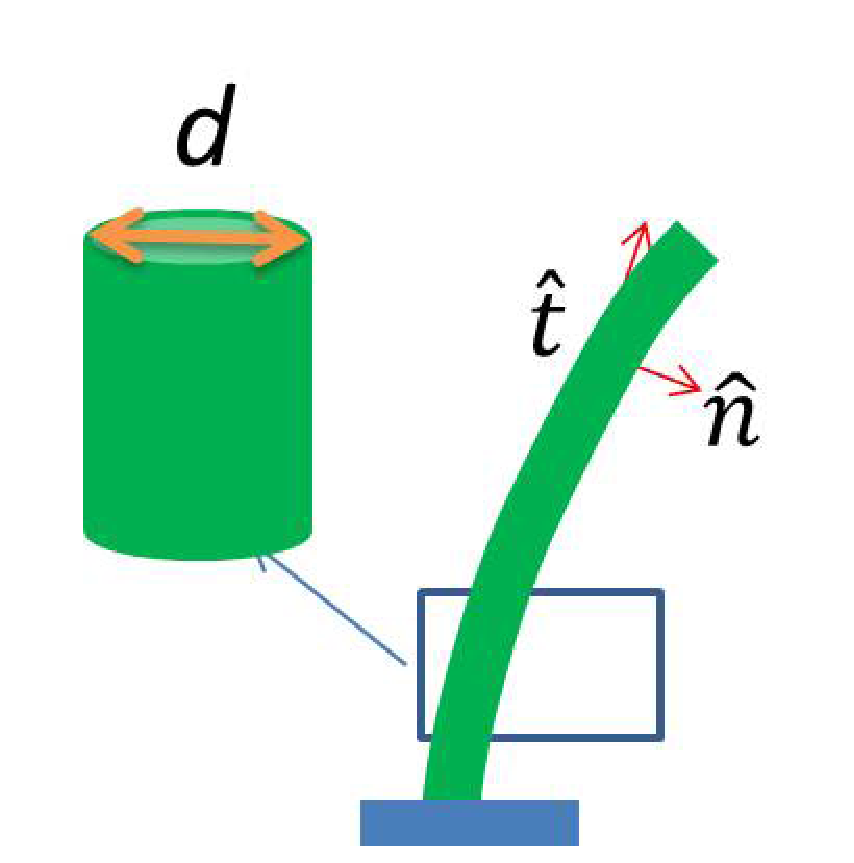
\includegraphics[width=4.0cm,height=4.0cm]{Grass_orientation}
\caption{Typical grass orientation}
\end{minipage}
\hspace{1.0cm}
\begin{minipage}[b]{5cm}
\centering
 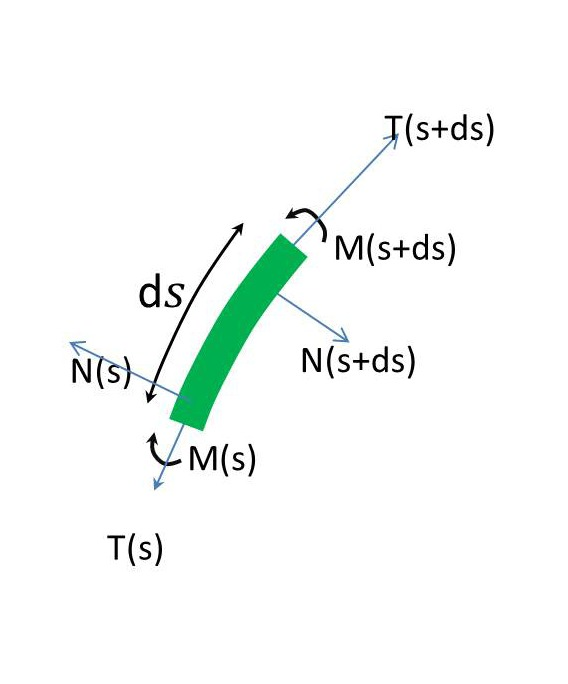
\includegraphics[width=5.0cm,height=5.5cm]{Grass_orientation2} 
\caption{Forces and moment on a section of grass}
\end{minipage}
\end{figure}
\end{center}
For flexible grass whose bending stiffness is really low, we assume that monami/honami is response to oscillations in flow velocity of fluid. In that case we can safely ignore
set of equation(3).
\section{Stability Analysis}
 In order to understand frequency and wavelength associated with passage of dominant eddies over grass which are manifestation of instability of mean flow 
in presence of grass, we investigate stability of base state obtained through equation of motion. We consider small perturbations $u, v, p$  associated 
with base profile $U$ and $P$ respectively. Momentum and mass balance equation expanded in 1st order of perturbed variable yields.
\begin{equation}
\begin{split}
 \frac{\del u}{\del t}+U\frac{\del u}{\del x}+v\frac{\del U}{\del y} &= -\frac{1}{\rho}\frac{\del p}{\del x}+\frac{\mu}{\rho}(u_{xx}+u_{yy})-2C_{N}dN_{g}Uu\\
 \frac{\del v}{\del  t}+ U\frac{\del v}{\del x} &= -\frac{1}{\rho}\frac{\del p}{\del y}+\frac{\mu}{\rho}(v_{xx}+v_{yy})\\
 \nabla\cdot \bu &= 0
\end{split}
\end{equation}
In most of recent work on honami/monami base profile have been approximated to a plane mixing layer profile having inflection point near top of canopy, It is also argued that 
It is instability associated with inflection of mean velocity which is responsible for coherent eddies traveling on top of canopies. In our calculation we get base velocity
profile by hydrodynamic balance between pressure, drag and diffusive force which also results in a velocity profile with inflection point near top of canopy with additional property 
of having been produced through equation of motion itself.\newline
We performed stability analysis on two different kind of base flow namely 1) flow driven by constant pressure gradient between two parallel plate  2) constant pressure gradient driven 
flow with zero shear at top. We use following scaling to non-dimensionlize equation of motion
   \[ u = U_{0}\bar{u},\hspace{1cm} y = (H/2)\bar{y}, \hspace{1cm} \text{with}\hspace{2mm} U_{0}=\frac{c_{1}H^2}{4\mu} \]
where $c_{1}$ is constant pressure gradient, H is height at which fluid is present. With these scaling and using stream function $\psi$ with $u = \psi_{y}, v= -\psi_x$, equations 
can be simplified into a single equation.
\begin{equation}
\begin{split}
 R_{e}\left[\psi_{yyt}+\psi_{xxt}+U\left(\psi_{xyy}+\psi_{xxx}\right)-U_{yy}\psi_{x} \right] &=\left[\psi_{yyxx}+\psi_{yyyy}+\psi_{xxxx}+\psi_{xxyy} \right]\\
& + 2D_{drag}U\psi_{y}\delta(y-h)\\
& - 2D_{drag}U_{y}\psi_{y} -2D_{drag}U\psi_{yy}
\end{split}
\end{equation}
where $R_{e}= \frac{\rho U_0 H}{2\mu}$ is Reynolds number and $\bar{N_g} = C_N d N_g H/2$ is non-dimensional grass number density and  $D_{drag} = R_{e}\bar{N_{g}}$ is non-dimensional drag
 seeking wave solution in form $\left(u,v,\psi \right)= \left(\hat u, \hat v, \hat\phi \right)e^{ikx+\sigma}$, we get modified orr-sommerfield equation which is an eigenvalue problem
whose solution will provide frequency and wavelength of eddies traveling over canopy.
\begin{equation}
\begin{split}
\sigma \left(D^2-k^2\phi \right) &= \frac{1}{R_{e}}\left[D^4\phi -2k^{2}D^2\phi +k^{4}\phi \right]\\
				  & +ikU_{yy}\phi-ikU\left(D^2\phi-k^2\phi \right)\\
 & -\frac{2D_{drag}}{R_{e}}U_{y}\phi_{y}-\frac{2D_{drag}}{R_{e}}U\phi_{yy}+\frac{2D_{drag}}{R_{e}}U\phi_{y}\delta(y-h)
\end{split}
\end{equation}
critical Reynolds number above which we get growing solution of perturbation, as a function of grass number density for different grass height shows following characteristics 
  \begin{figure}[htb!]
  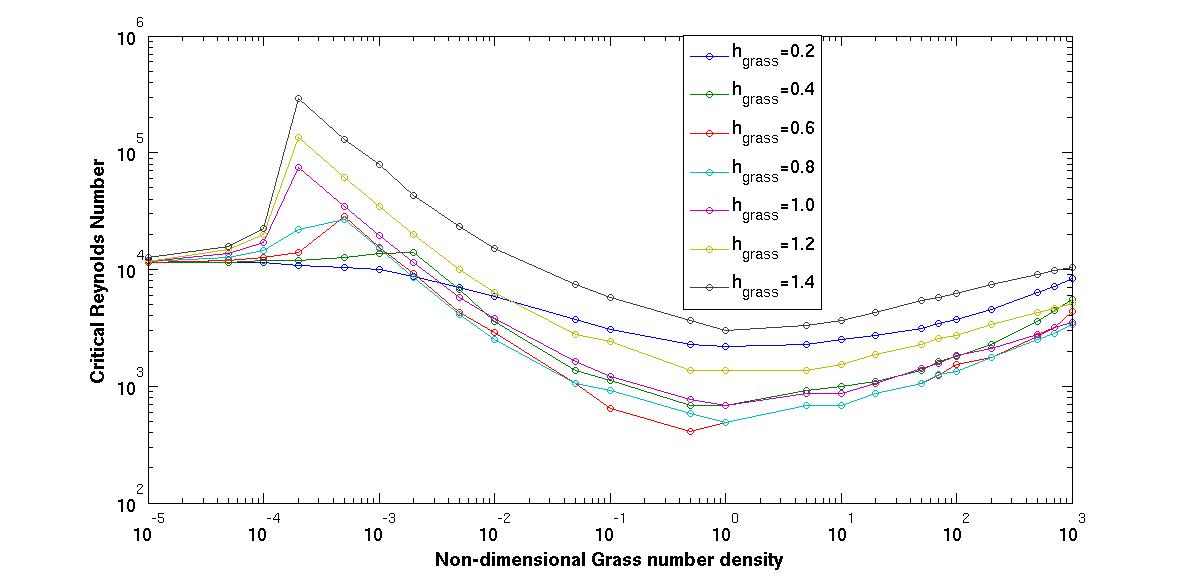
\includegraphics[scale=0.35]{Instability2}
\caption{Critical Reynolds number with flow between parallel plate for different grass height as a function of grass number density}
\end{figure}

\begin{figure}[htb!]
  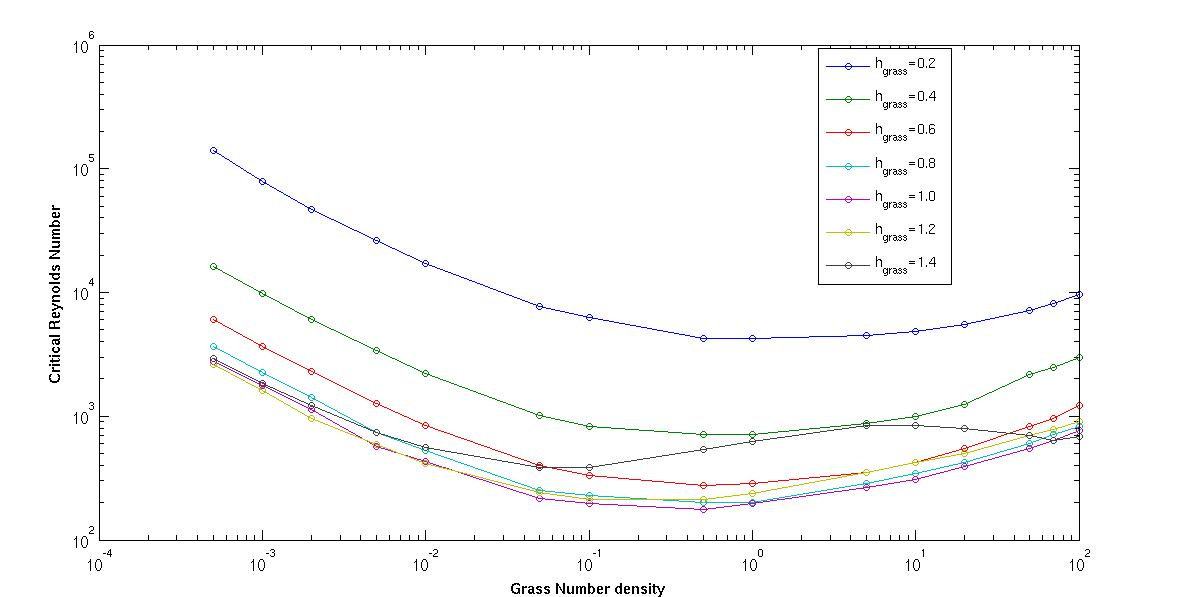
\includegraphics[scale=0.35]{Instability1_free.jpg}
\caption{Critical Reynolds number with no shear stress at top for different grass height as a function of grass number density}
\end{figure}

\end{document}
